\begin{figure}[htpb]
	\centering\capstart{}
	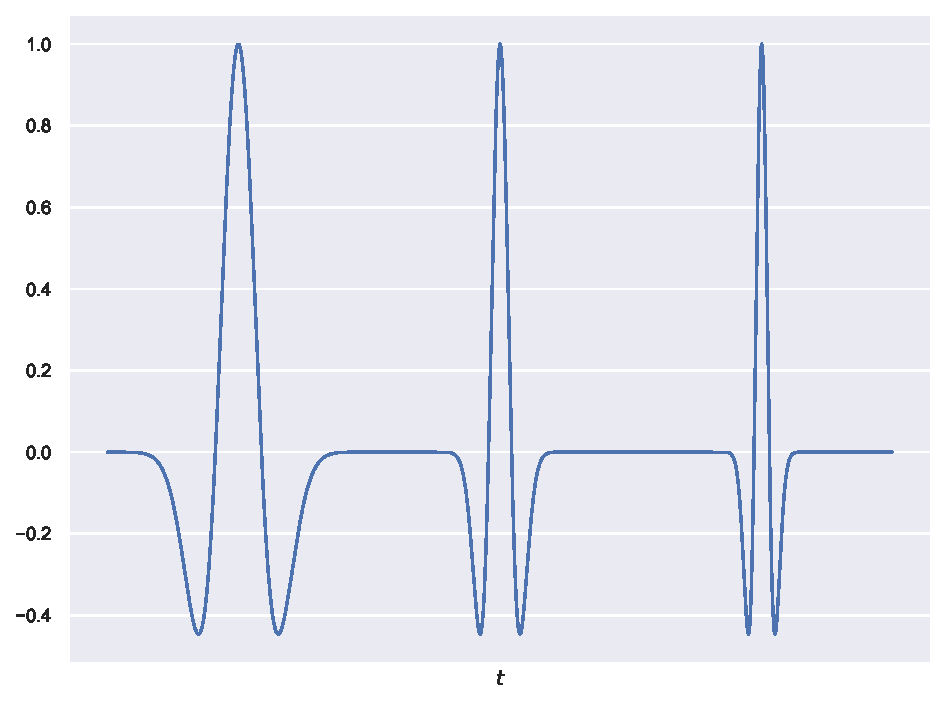
\includegraphics[width=\textwidth]{ricker_wavelets.pdf}
	\caption[
        A few Ricker wavelets
	]{
        Some Ricker wavelets~\cite{Ricker1953} (also known as Mexican hat wavelets) shown alongside each other on the time axis.
        These wavelets arise as the second derivative of the Gaussian function.
        In wavelet analyses, a (Euclidean) signal is probed with many differently sized wavelets.
	}\label{fig:chapter2_ricker_wavelets}
\end{figure}
